\documentclass[conference]{IEEEtran}

\usepackage[T1]{fontenc}
\usepackage[utf8]{inputenc}
\usepackage{lmodern}
\usepackage{graphicx}
\usepackage{booktabs}
\usepackage{array}
\usepackage{amsmath}
\usepackage{amssymb}
\usepackage{hyperref}
\usepackage{microtype}
\usepackage{xcolor}
\setlength{\textfloatsep}{8pt plus 1pt minus 2pt}
\setlength{\floatsep}{6pt plus 1pt minus 2pt}
\setlength{\intextsep}{8pt plus 1pt minus 2pt}
\setlength{\abovecaptionskip}{4pt}
\setlength{\belowcaptionskip}{0pt}

\hypersetup{
  colorlinks=true,
  linkcolor=blue!50!black,
  citecolor=blue!50!black,
  urlcolor=blue!50!black
}

\title{Lexical and LLM-Based Representations for Public Tender Outcome Prediction: A Comparative Study}
\author{}

\begin{document}
\maketitle

\begin{abstract}
This short paper examines public tender outcome prediction as a comparison between lexical and LLM-based document representations. Each example corresponds to one procurement paired with the text of its bidding document (\emph{Pliego de Bases y Condiciones}, PBC). We compare five model families: dummy baselines, TF--IDF with logistic regression, mean-pooled LLM chunk embeddings with logistic regression, mean-pooled LLM chunk embeddings with a small multilayer perceptron, and a lightweight transformer over LLM chunk embeddings. Labels are derived from final procurement status, mapping \texttt{complete} to successful outcome and \texttt{unsuccessful}/\texttt{cancelled}/\texttt{canceled} to non-successful outcome. The dataset is derived from public procurement data published in Paraguay and focuses on road construction tenders.

The experiments use a procurement snapshot containing 10{,}628 records, from which a processed supervised subset of 1{,}162 procurements was obtained after document availability, text extraction, and embedding-generation filtering. On this subset, TF--IDF with logistic regression provides the strongest ranking performance, reaching mean ROC AUC 0.814 and mean PR AUC 0.899 under deterministic stratified 5-fold cross-validation. The cross-chunk transformer over LLM embeddings does not improve ranking over the strongest lexical baseline, but it achieves the best calibration, with mean Brier score 0.162, and shows the greatest stability under threshold tuning. Mean-pooled embedding baselines remain close to the transformer, suggesting that much of the useful signal is already present in the frozen chunk embeddings.

Methodologically, the models operate exclusively on bidding documents that are produced and published during the call-for-tender stage, so the inputs reflect information available at inference time. This reduces the risk of direct leakage from post hoc outcome content. The remaining concerns are indirect predictive correlations, selection bias from the processed subset, and mismatch between the experimental class balance and the more imbalanced real-world population. The contribution of this study is therefore empirical and analytical: it clarifies how predictive signal in this task is distributed across lexical features, dense pretrained representations, calibration behavior, and threshold sensitivity.
\end{abstract}

\begin{IEEEkeywords}
public procurement, tender documents, large language models, transfer learning, outcome prediction, document classification
\end{IEEEkeywords}

\section{Introduction}
Public procurement processes are strongly shaped by the content of bidding documents, which define administrative conditions, technical requirements, qualification rules, and delivery constraints. These documents may contain information associated with the eventual success or failure of the procurement process. Such information need not be causal to be useful for prediction. The relevant question is therefore not only whether tender outcomes can be predicted from document text, but also which representation of that text is most informative.

This paper studies that question through a direct comparison between sparse lexical features and LLM-based dense representations. The analysis focuses on road construction tenders, whose bidding documents are often relatively structured and standardized. Sparse lexical models remain strong and interpretable baselines in document classification \cite{wang2012baselines,joulin2017bag}, while pretrained language models offer flexible dense representations for long and heterogeneous text \cite{yang2016han,beltagy2020longformer,zaheer2020bigbird}. In the present setting, the goal is not to establish a universally superior model family, but to understand how much predictive signal can be recovered from lexical cues, how much is already captured in frozen dense embeddings, and whether explicit cross-chunk modeling provides additional value.

Our pipeline uses a pretrained causal LLM as a frozen encoder to produce chunk-level embeddings from Spanish tender documents. We compare two simple aggregation strategies over these embeddings, based on mean pooling, against a lightweight transformer that models cross-chunk interactions. These LLM-based approaches are evaluated alongside TF--IDF plus logistic regression and trivial dummy baselines. This design makes it possible to separate representation effects from downstream modeling effects.

The contribution of this short paper is empirical rather than competitive. It provides a reproducible comparison across lexical, dummy, pooled-embedding, and cross-chunk transformer baselines under deterministic 5-fold cross-validation. It also analyzes ranking performance, calibration, and threshold sensitivity separately. The central result is nuanced: TF--IDF plus logistic regression is the strongest ranking model, while the cross-chunk transformer offers the best calibration and the most stable behavior under threshold changes. This is useful evidence for the broader question of how textual signal is distributed in public tender documents.

\section{Task Definition}
The prediction task is binary classification over procurements for which both a usable bidding document and an outcome label are available. Each example corresponds to one procurement process paired with one extracted PBC document. The target variable is operationalized from the procurement status field as follows:

\begin{itemize}
  \item Successful outcome ($y=1$): \texttt{complete}
  \item Non-successful outcome ($y=0$): \texttt{unsuccessful}, \texttt{cancelled}, or \texttt{canceled}
\end{itemize}

Records with other statuses are excluded from supervised training and evaluation. This definition is intentionally simple and directly grounded in the available data source. It should be understood as an operational proxy for procurement success rather than as an exhaustive institutional notion of performance.

\section{Method}
\subsection{Document Representation}
Each PBC document is first converted from PDF to text by the upstream extraction pipeline. The resulting text is tokenized and split into overlapping chunks. In the current implementation, the chunk length is 4096 tokens with a stride of 2048 tokens. A pretrained causal language model, \texttt{openai/gpt-oss-20b}, is used as a frozen document encoder. Chunks are processed in micro-batches to reduce GPU memory pressure.

For every chunk, the system extracts the hidden representation associated with the last valid token. The output for one procurement document is therefore a sequence of chunk embeddings:
\[
\mathbf{E} = [\mathbf{e}_1, \mathbf{e}_2, \dots, \mathbf{e}_N], \qquad \mathbf{e}_i \in \mathbb{R}^{d_{in}},
\]
where $N$ is the number of chunks in the document and $d_{in}$ is determined by the hidden size of the pretrained model. This setup makes it possible to compare two LLM-based representation strategies: a simple document vector obtained by mean pooling over chunks, and a sequence model that learns interactions across chunks.

\subsection{Predictor Architecture}
The main downstream classifier, \texttt{TenderSuccessPredictor}, is a lightweight transformer over chunk embeddings. Let $\mathbf{E} \in \mathbb{R}^{N \times d_{in}}$ denote the chunk sequence of a document. The model applies:

\begin{enumerate}
  \item A linear projection from $d_{in}$ to a trainable latent dimension $d_{model}$.
  \item The insertion of a learned \texttt{[CLS]} token at the beginning of the sequence.
  \item A transformer encoder over the full sequence of chunk vectors.
  \item A small multilayer classification head on top of the final \texttt{[CLS]} representation.
\end{enumerate}

In the current experiments, the downstream hyperparameters are: $d_{model}=128$, $n_{heads}=4$, feed-forward dimension $=512$, dropout $=0.3$, and one encoder layer. Padding masks are used so that different numbers of chunks can be batched together safely.

The model outputs a single logit per document. A sigmoid transformation converts this logit into a probability of success:
\[
\hat{p}(y=1 \mid \mathbf{E}) = \sigma(z).
\]
Training uses binary cross-entropy with logits.

\subsection{Baselines}
To interpret the LLM-based results, we evaluate three classes of baselines.

First, we use two dummy references: a majority-class classifier and a random classifier with positive rate matched to the empirical class prevalence. These baselines establish the expected no-skill region, where ROC AUC should be near $0.5$ and PR AUC should be near the positive prevalence.

Second, we use a lexical baseline based on TF--IDF features with up to 50{,}000 unigram and bigram features, minimum document frequency $5$, and a logistic-regression classifier with balanced class weights. Linear bag-of-words baselines of this kind are standard, strong references in text classification \cite{wang2012baselines,joulin2017bag}.

Third, we define two intermediate LLM baselines using the same pretrained chunk embeddings as the main system but replacing the cross-chunk transformer with simpler document-level aggregation. In the first variant, chunk embeddings are mean-pooled and fed to logistic regression. In the second, the same mean-pooled representation is fed to a small multilayer perceptron with one hidden layer. These baselines isolate the value of the representation from the value of explicit cross-chunk interaction modeling.

\subsection{Training and Reproducibility}
Training is performed with AdamW, learning rate $10^{-4}$, weight decay $0.01$, batch size $8$, and up to $50$ epochs. Early stopping monitors validation loss with patience set to $5$, and the best validation checkpoint is restored at the end of each fold.

Because this study is intended for academic reporting, reproducibility is treated as a first-class concern. The training script fixes seeds for Python, NumPy, and PyTorch; configures deterministic cuDNN behavior; uses a fixed random generator for the training dataloader; and reinitializes the random state independently at the beginning of every fold. As a result, repeated runs with the same seed, data, and software environment are expected to produce the same splits and the same training trajectory, modulo rare low-level differences across hardware or driver stacks.

\section{Experimental Setup}
\subsection{Dataset}
The metadata snapshot used in this paper was constructed from public procurement records published by the Dirección Nacional de Contrataciones Públicas (DNCP) of Paraguay and retrieved through the official open-data API endpoint \texttt{v3/doc/search/processes}. The initial query restricted the sample to processes with status \texttt{complete} and to items classified under catalog code \texttt{72131701}, which corresponds to the road construction and paving domain. The resulting dataset is therefore domain-specific to road construction tenders and combines structured procurement metadata with associated PDF documents, including PBC files and additional public documents from the same source used to support labeling. The full snapshot contains 10{,}628 procurement records in an OCDS-like schema, together with references to associated PBC files.

The supervised subset used for modeling is smaller because several filtering steps are required: a procurement must have an available PBC, successful text extraction, precomputed embeddings, and a status belonging to the final binary target classes. After applying these constraints, the effective dataset contains 1{,}162 examples. The collection process was automated rather than manually curated, and the final filtering was driven primarily by time and budget constraints in document extraction and processing rather than by a sampling design targeted at representativeness. The conclusions of the present study therefore apply to the processed subset rather than automatically to the full procurement population.

Class distribution in the processed subset is moderately imbalanced: 844 procurements ($72.63\%$) are labeled as successful (\texttt{complete}) and 318 ($27.37\%$) as non-successful (\texttt{unsuccessful}/\texttt{cancelled}/\texttt{canceled}). The average represented document length is 7.46 chunks per procurement, with a standard deviation of 13.52, a median of 3 chunks, and a maximum of 245 chunks. These values indicate a highly skewed length distribution, with many short documents and a smaller number of substantially longer documents. The embedding dimension inherited from the frozen base LLM is 2880.

The processed subset is also less imbalanced than the broader procurement population. In the full snapshot, successful outcomes are much more frequent, on the order of roughly 10{,}000 successful versus about 650 non-successful procurements. Threshold-dependent metrics and prevalence-sensitive interpretations should therefore be understood as valid for the processed subset and not as directly deployable operating points.

\subsection{Leakage Handling}
The model operates exclusively on information available at inference time. All inputs are derived from bidding documents that are produced and published during the call-for-tender stage, before the final procurement outcome is known. This makes the prediction setup operationally realistic and substantially reduces the risk of direct leakage from explicit final-status content.

Accordingly, the main remaining validity concern is not obvious post hoc target leakage. Rather, the more plausible concerns are indirect predictive correlations and limited representativeness. Tender documents may encode structural, institutional, or stylistic regularities that are predictive of outcome without being causal in themselves. Such regularities are legitimate for ex ante prediction because they are available at decision time, but they should not be interpreted as direct causal drivers of procurement success or failure.

\subsection{Evaluation Protocol}
The model is evaluated with stratified 5-fold cross-validation. This choice reflects a standard trade-off between robustness of performance estimates and computational cost. Stratification is important here because the positive class is not balanced: approximately 72.6\% of the validation examples correspond to successful outcomes. By preserving class proportions across folds, the protocol reduces unnecessary variance in threshold-sensitive metrics such as F1-score, balanced accuracy, and PR AUC.

For each fold, the model is trained on four partitions and evaluated on the held-out partition. The final reported values are the mean and standard deviation across folds. This reporting strategy is preferable to a single train/test split for a preliminary study because it reduces dependence on an arbitrary partition. In a second analysis, threshold sensitivity is examined by selecting, inside each outer training fold, an inner validation split on which the probability threshold is tuned to maximize F1; this tuned threshold is then evaluated on the held-out outer test fold.

\subsection{Metrics}
The evaluation uses the following metrics:

\begin{itemize}
  \item \textbf{ROC AUC}, to measure ranking quality independently of the decision threshold.
  \item \textbf{PR AUC} (average precision), to assess ranking quality with explicit attention to the positive class.
  \item \textbf{F1-score}, using a probability threshold of 0.5.
  \item \textbf{Balanced accuracy}, also with threshold 0.5.
  \item \textbf{Brier score}, to measure probabilistic calibration quality.
  \item \textbf{Log loss}, as a proper scoring rule over predicted probabilities.
\end{itemize}

Because PR AUC can be misleading when the positive class is frequent, it is interpreted together with the positive prevalence $\pi$ in the validation folds. In the current implementation, the system therefore also logs \texttt{positive\_prevalence} and \texttt{pr\_auc\_excess\_over\_prevalence}, where the latter is defined as PR AUC minus $\pi$. This quantity provides a compact estimate of how much the model improves over the positive-class frequency as a reference level commonly used when discussing no-skill PR behavior in imbalanced settings.

\section{Results}
\subsection{Ranking Performance}
Table~\ref{tab:main-results} summarizes the model comparison. The dummy baselines behave as expected: ROC AUC remains at chance level and PR AUC stays close to the positive prevalence of approximately $0.726$. This provides a useful no-skill reference and supports the internal consistency of the evaluation setup.

Among the non-trivial models, TF--IDF plus logistic regression yields the strongest ranking metrics, with mean ROC AUC $0.814$ and mean PR AUC $0.899$. The cross-chunk transformer over LLM embeddings reaches ROC AUC $0.755$ and PR AUC $0.886$, while the mean-pooled embedding baselines remain close: mean-pooled MLP reaches ROC AUC $0.763$ and PR AUC $0.894$, and mean-pooled logistic regression reaches ROC AUC $0.758$ and PR AUC $0.881$. Fig.~\ref{fig:pr} is consistent with this ranking picture: TF--IDF defines the strongest precision-recall frontier overall, while both LLM-based alternatives remain clearly above the prevalence baseline. The documents therefore do contain predictive signal, but the strongest ranking performance in the current setup comes from lexical rather than dense representations.

\subsection{Threshold Sensitivity}
Threshold-sensitive behavior reveals a different pattern. At the default threshold of $0.5$, the cross-chunk transformer attains the highest F1-score ($0.858$ in the original 5-fold evaluation). However, the dedicated threshold-sensitivity experiment shows that not all models react similarly to threshold optimization. For TF--IDF plus logistic regression, selecting the validation threshold that maximizes F1 increases test-fold F1 by $0.103$ on average, but does not improve balanced accuracy on average. Mean-pooled logistic regression shows only a modest F1 gain ($+0.014$) and a mean decrease in balanced accuracy ($-0.049$). By contrast, the cross-chunk transformer changes little under threshold tuning (mean $\Delta$F1 $=+0.002$, mean $\Delta$ balanced accuracy $=+0.002$), suggesting that the default threshold of $0.5$ is already near a stable operating point. The mean-pooled MLP is intermediate: its F1 barely changes, but its balanced accuracy improves on average when the threshold is tuned. Fig.~\ref{fig:threshold-sensitivity} summarizes this contrast visually and makes clear that threshold optimization mostly benefits the lexical model's F1 rather than all models uniformly.

\subsection{Calibration}
Calibration tells a different story from ranking. The cross-chunk transformer achieves the best Brier score ($0.162$), followed by the mean-pooled MLP ($0.165$), while TF--IDF plus logistic regression is weaker ($0.179$) and mean-pooled logistic regression is substantially worse ($0.201$). This pattern indicates that lexical features can be highly effective for ranking examples, but that LLM-based dense representations provide more reliable probabilities. Fig.~\ref{fig:calibration} is consistent with this interpretation: among the three most informative model families, the transformer remains closest to the diagonal across much of the probability range, while TF--IDF shows stronger ranking than calibration. This matters because model selection in public-procurement monitoring may depend not only on ranking but also on whether predicted probabilities can support downstream triage or risk scoring \cite{guo2017calibration}.

\subsection{Representation Comparison}
The comparison between mean-pooled embeddings and the cross-chunk transformer is informative in its own right. If the main value of the LLM representation came only from cross-chunk interactions, one would expect the transformer to dominate the mean-pooled baselines. That does not happen. Mean-pooled MLP slightly exceeds the transformer on ROC AUC and PR AUC, while mean-pooled logistic regression achieves substantially higher balanced accuracy. These results suggest that a large fraction of the predictive information is already encoded in the frozen chunk embeddings themselves, and that explicit cross-chunk modeling provides only limited gains in the current setup. The main advantage of the transformer appears to be calibration and stable threshold behavior rather than clearly superior ranking.

\begin{table}[t]
\centering
\caption{Model comparison under 5-fold cross-validation (mean $\pm$ standard deviation). Lower is better for Brier score; higher is better for the remaining metrics.}
\label{tab:main-results}
\footnotesize
\begin{tabular}{>{\raggedright\arraybackslash}p{0.46\linewidth} >{\raggedleft\arraybackslash}p{0.20\linewidth}}
\toprule
Metric & Value \\
\midrule
Dummy majority: ROC AUC / PR AUC & 0.500 / 0.726 \\
Dummy random: ROC AUC / PR AUC & 0.493 / 0.724 \\
TF--IDF + LogReg: ROC AUC / PR AUC & 0.814 / 0.899 \\
TF--IDF + LogReg: F1 / Bal. Acc. / Brier & 0.790 / 0.728 / 0.179 \\
MeanPool + LogReg: ROC AUC / PR AUC & 0.758 / 0.881 \\
MeanPool + LogReg: F1 / Bal. Acc. / Brier & 0.843 / 0.704 / 0.201 \\
MeanPool + MLP: ROC AUC / PR AUC & 0.763 / 0.894 \\
MeanPool + MLP: F1 / Bal. Acc. / Brier & 0.849 / 0.604 / 0.165 \\
Cross-chunk transformer: ROC AUC / PR AUC & 0.755 / 0.886 \\
Cross-chunk transformer: F1 / Bal. Acc. / Brier & 0.858 / 0.636 / 0.162 \\
\bottomrule
\end{tabular}
\end{table}

\begin{table}[t]
\centering
\caption{Threshold tuning on an inner validation split and evaluation on the outer test fold. Reported values are means across folds.}
\label{tab:thresholds}
\begin{tabular}{>{\raggedright\arraybackslash}p{0.44\linewidth} >{\raggedleft\arraybackslash}p{0.22\linewidth}}
\toprule
Metric & Value \\
\midrule
TF--IDF + LogReg: $\Delta$F1 / $\Delta$ Bal. Acc. & $+0.103 / -0.008$ \\
MeanPool + LogReg: $\Delta$F1 / $\Delta$ Bal. Acc. & $+0.014 / -0.049$ \\
MeanPool + MLP: $\Delta$F1 / $\Delta$ Bal. Acc. & $+0.002 / +0.053$ \\
Cross-chunk transformer: $\Delta$F1 / $\Delta$ Bal. Acc. & $+0.002 / +0.002$ \\
\bottomrule
\end{tabular}
\end{table}

\begin{figure}[t]
  \centering
  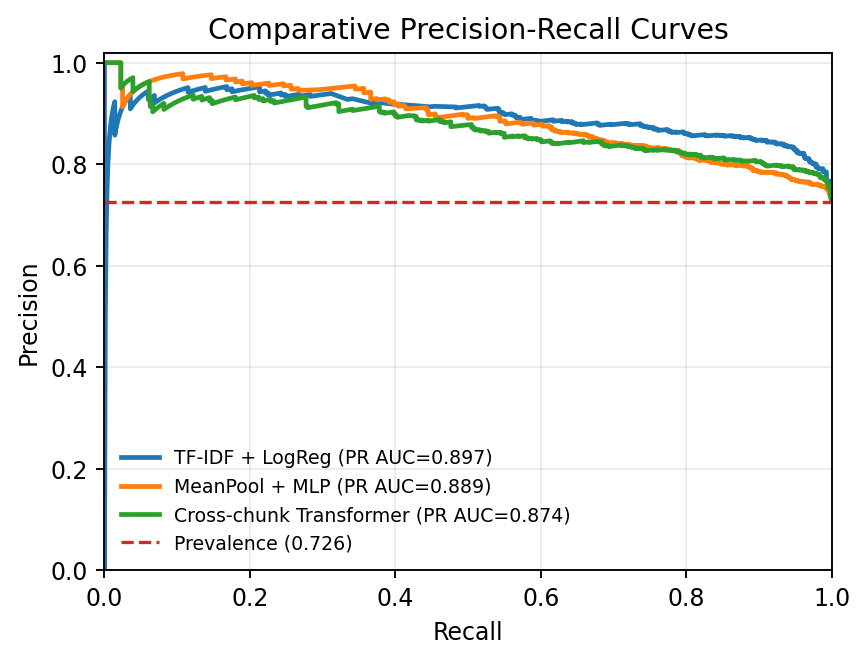
\includegraphics[width=\linewidth]{figures/pr_curve_cv.png}
  \caption{Comparative precision-recall curves from pooled out-of-fold predictions for the strongest lexical baseline (TF--IDF + logistic regression), the strongest mean-pooled dense baseline (MeanPool + MLP), and the cross-chunk transformer. The dashed horizontal line marks the positive prevalence baseline ($\pi \approx 0.726$). TF--IDF shows the strongest precision-recall trade-off overall, while both LLM-based models remain substantially above the no-skill baseline.}
  \label{fig:pr}
\end{figure}

\begin{figure}[t]
  \centering
  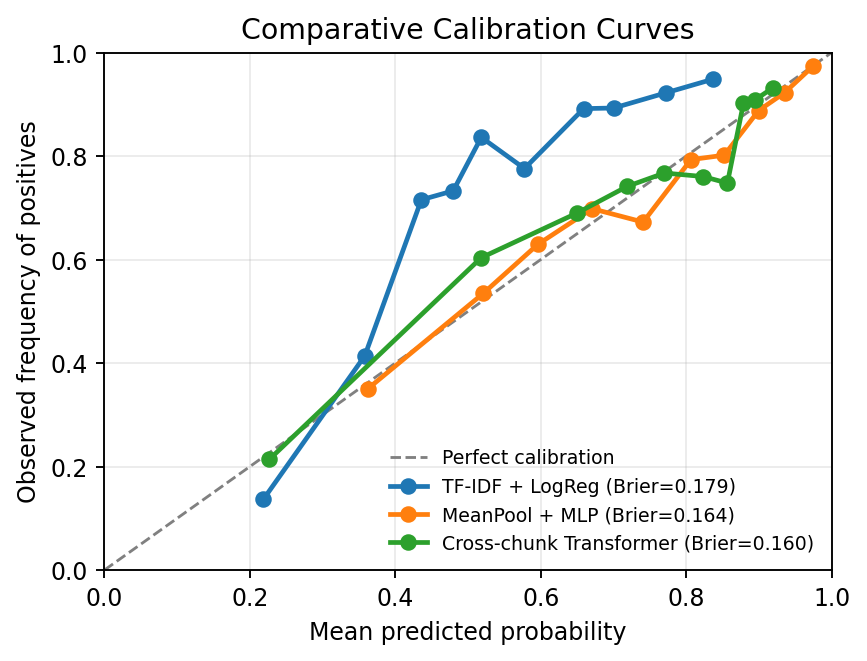
\includegraphics[width=\linewidth]{figures/calibration_curve_cv.png}
  \caption{Comparative calibration curves from pooled out-of-fold predictions for TF--IDF + logistic regression, MeanPool + MLP, and the cross-chunk transformer. The diagonal line indicates perfect calibration. Ranking and calibration do not coincide: the transformer remains closest to a useful calibrated probability signal, while TF--IDF is stronger as a ranking model than as a probability estimator.}
  \label{fig:calibration}
\end{figure}

\begin{figure}[t]
  \centering
  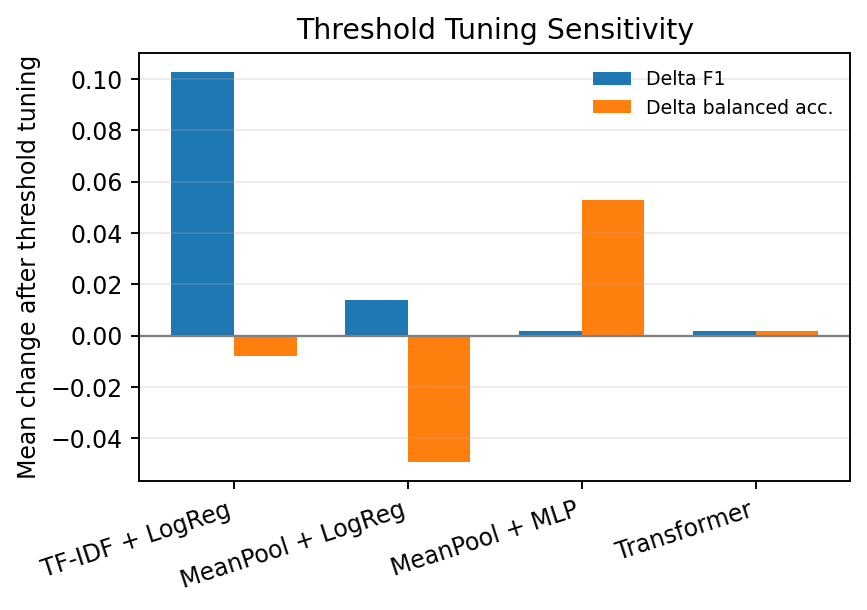
\includegraphics[width=\linewidth]{figures/threshold_sensitivity_comparison.png}
  \caption{Mean change in test-fold F1 and balanced accuracy after replacing the default threshold of $0.5$ with the F1-maximizing threshold selected on an inner validation split. Threshold tuning strongly improves F1 for TF--IDF + logistic regression, has mixed effects for mean-pooled models, and changes the cross-chunk transformer only marginally, indicating greater operating-point stability.}
  \label{fig:threshold-sensitivity}
\end{figure}

\section{Discussion}
The main finding is not that one representation universally dominates the others, but that different representations appear to capture different aspects of the task. TF--IDF plus logistic regression delivers the best ranking performance, which suggests that lexical signal is highly informative in this domain. This is plausible because tender documents often contain repeated administrative formulas, standardized requirements, domain-specific terminology, and procedural phrasing that can correlate strongly with downstream outcomes. In such a setting, sparse lexical features can recover a large share of the predictive signal with a relatively simple linear model.

This should not be interpreted as evidence against LLM-based representations. All non-trivial LLM-based models remain well above the dummy baselines, and the mean-pooled embedding baselines stay close to the cross-chunk transformer. This indicates that the frozen chunk embeddings already encode useful dense information. In other words, much of the value of the LLM may lie in the representation itself rather than in the complexity of the downstream aggregation mechanism.

The comparison between mean pooling and the cross-chunk transformer is especially informative. If fine-grained cross-chunk interactions were the primary source of predictive power, the transformer should clearly dominate the pooled baselines. That does not occur in the current experiments. Mean-pooled MLP is close to the transformer in ranking, and mean-pooled logistic regression even exceeds it in balanced accuracy. This suggests that explicit cross-chunk interaction modeling does not yet provide a clear ranking advantage under the present data regime and supervision signal.

The cross-chunk transformer nevertheless retains an important advantage: calibration and threshold stability. It achieves the best Brier score and shows very small sensitivity to threshold tuning, while TF--IDF plus logistic regression benefits strongly from threshold tuning for F1. From an applied perspective, this matters because a model preferred for ranking is not necessarily the same model preferred for probability-based triage or stable deployment behavior. The relatively standardized nature of road construction tender documents may also contribute to the strong performance of lexical baselines in this setting.

Some of the predictive signal may reflect document complexity, institutional writing practices, procedural standardization, or other latent textual regularities. Such signals are legitimate for prediction because they are available ex ante, at the time the document is issued. However, they should not be interpreted as causal drivers of procurement outcomes.

Overall, the comparison is informative even without a single dominant winner. It shows that lexical models are very competitive in this domain, that frozen LLM embeddings already capture much of the useful dense signal, and that the principal comparative advantage of the transformer lies in calibration and threshold stability rather than in raw ranking performance.

\section{Limitations}
Several limitations should qualify the interpretation of these results. First, the supervised dataset is a processed subset rather than a representative sample of the full procurement population. Inclusion required document availability, successful text extraction, successful embedding generation, and one of the two final target statuses. Because this filtering was driven mainly by time and budget constraints in extraction and processing, the conclusions should be understood as applying to the processed subset.

Second, the processed subset is less imbalanced than the real-world procurement population. The experimental data contain roughly $73\%$ positive examples, whereas the broader population is much more skewed toward successful outcomes, on the order of roughly $94\%$ positive. This difference matters because threshold-dependent metrics and prevalence-sensitive interpretations are not invariant to class balance. Reported operating points should therefore not be treated as directly deployable without recalibration in the target environment.

Third, threshold non-transferability is a practical concern. Validation-optimized thresholds improve some metrics in the present sample, especially for TF--IDF plus logistic regression, but those thresholds may shift under different prevalences, institutional settings, or error-cost assumptions. Threshold tuning should therefore be interpreted as an analysis tool for this dataset rather than as a universal prescription.

Fourth, the main residual concern is not direct leakage from final outcome information. Because the documents are produced during the call-for-tender stage, such direct leakage appears unlikely. The more relevant risks are indirect predictive correlations, shortcut learning, limited representativeness, and distribution mismatch. For example, models may exploit institutional or stylistic regularities that are predictive in this dataset but less stable across agencies, periods, or procurement categories. The findings may also be domain-specific to road construction procurement and may not transfer unchanged to other procurement categories.

\section{Conclusion}
This short paper presented a comparative study of lexical and LLM-based representations for public procurement outcome prediction from bidding documents. The results show that tender documents contain substantial predictive signal, but they also show that the strongest ranking model in the current setting is a classical lexical baseline, TF--IDF plus logistic regression. At the same time, the cross-chunk transformer over LLM embeddings achieves the best calibration and the strongest stability under threshold changes.

The comparison also indicates that much of the useful dense signal is already present in the frozen chunk embeddings, since mean-pooled embedding baselines remain close to the transformer. This suggests that explicit cross-chunk interaction modeling does not currently provide a clear ranking advantage, although it may still offer practical value through more reliable probability estimates and more stable decision behavior.

The main contribution of the study is therefore empirical and interpretive. It shows that lexical features capture a large share of the predictive signal in this domain, that pretrained dense representations remain useful, and that ranking quality, calibration, and threshold sensitivity should be analyzed separately. These findings provide a more precise basis for understanding what current tender-document models are learning and how their behavior should be interpreted under realistic deployment constraints.

\begin{thebibliography}{10}

\bibitem{devlin2019bert}
Jacob Devlin, Ming-Wei Chang, Kenton Lee, and Kristina Toutanova.
\newblock BERT: Pre-training of Deep Bidirectional Transformers for Language Understanding.
\newblock In \emph{Proceedings of NAACL-HLT}, 2019.

\bibitem{radford2019language}
Alec Radford, Jeffrey Wu, Rewon Child, David Luan, Dario Amodei, and Ilya Sutskever.
\newblock Language Models are Unsupervised Multitask Learners.
\newblock OpenAI Technical Report, 2019.

\bibitem{saito2015precision}
Takaya Saito and Marc Rehmsmeier.
\newblock The Precision-Recall Plot Is More Informative than the ROC Plot When Evaluating Binary Classifiers on Imbalanced Datasets.
\newblock \emph{PLOS ONE}, 10(3), 2015.

\bibitem{wang2012baselines}
Sida Wang and Christopher D. Manning.
\newblock Baselines and Bigrams: Simple, Good Sentiment and Topic Classification.
\newblock In \emph{Proceedings of ACL}, 2012.

\bibitem{joulin2017bag}
Armand Joulin, Edouard Grave, Piotr Bojanowski, and Tomas Mikolov.
\newblock Bag of Tricks for Efficient Text Classification.
\newblock In \emph{Proceedings of EACL}, 2017.

\bibitem{yang2016han}
Zichao Yang, Diyi Yang, Chris Dyer, Xiaodong He, Alex Smola, and Eduard Hovy.
\newblock Hierarchical Attention Networks for Document Classification.
\newblock In \emph{Proceedings of NAACL-HLT}, 2016.

\bibitem{beltagy2020longformer}
Iz Beltagy, Matthew E. Peters, and Arman Cohan.
\newblock Longformer: The Long-Document Transformer.
\newblock \emph{arXiv preprint arXiv:2004.05150}, 2020.

\bibitem{zaheer2020bigbird}
Manzil Zaheer, Guru Guruganesh, Kumar Avinava Dubey, Joshua Ainslie, Chris Alberti, Santiago Onta\~n\'on, Philip Pham, Anirudh Ravula, Qifan Wang, Li Yang, and Amr Ahmed.
\newblock Big Bird: Transformers for Longer Sequences.
\newblock In \emph{Advances in Neural Information Processing Systems}, 2020.

\bibitem{guo2017calibration}
Chuan Guo, Geoff Pleiss, Yu Sun, and Kilian Q. Weinberger.
\newblock On Calibration of Modern Neural Networks.
\newblock In \emph{Proceedings of ICML}, 2017.

\bibitem{caruana2006empirical}
Rich Caruana and Alexandru Niculescu-Mizil.
\newblock An Empirical Comparison of Supervised Learning Algorithms.
\newblock In \emph{Proceedings of ICML}, 2006.

\bibitem{goodfellow2016deep}
Ian Goodfellow, Yoshua Bengio, and Aaron Courville.
\newblock \emph{Deep Learning}.
\newblock MIT Press, 2016.

\end{thebibliography}

\end{document}
